\documentclass[adobefonts, nocap]{ctexart}
\usepackage{amsmath}
\usepackage{amsfonts}
\usepackage{listings}
\usepackage{xcolor}
\usepackage{graphicx}
\usepackage{siunitx}
\usepackage{hyperref}
\hypersetup{
  colorlinks = true,
  linkcolor = blue,
  unicode = true
}
\lstset{
  language = C++,
  basicstyle = \small\ttfamily,
  keywordstyle = \small\ttfamily\color{red},
  stringstyle = \color{gray},
  numbers = left,
  numberstyle = \small,
  numbersep = 5pt,
  frame = leftline,
  showstringspaces = false
}
\def\D{\mathrm{d}}
\begin{document}
  \title{计算机系统结构第三次作业}
  \author{李雨田\hspace{1em}2010012193\hspace{1em}计14}
  \maketitle
  \section*{3.8}
    如图所示,可以先计算$A_{i}\times B_{i}$, $i\in \{1,2,3\}$,在计算$A_{4}\times B_{4}$之前先计算出$A_{1}\times B_{1}+A_{2}\times B_{2}$,然后再算出剩下的值.

    \begin{center}
      \centering
      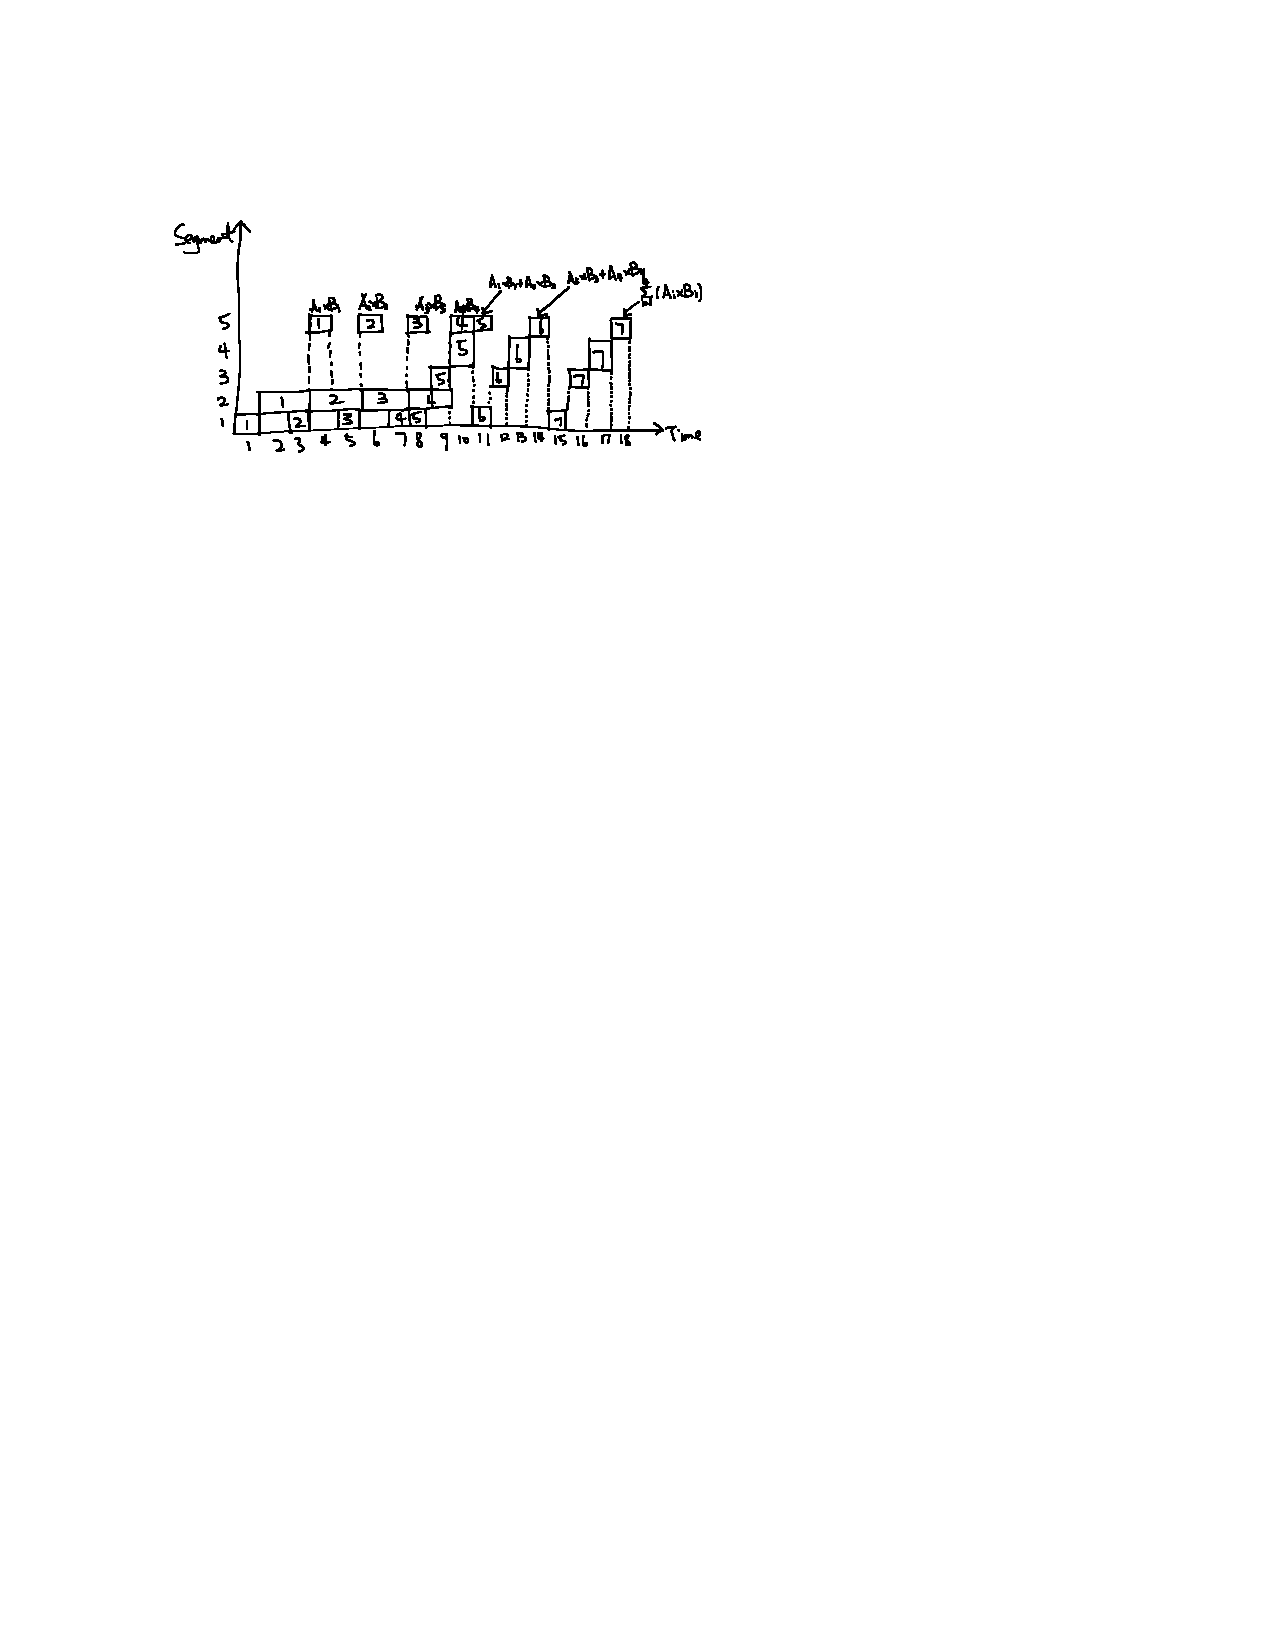
\includegraphics[width=10cm]{1-crop.pdf}
    \end{center}
    
    在$18$个$\Delta t$时间中,给出了$7$个结果,所以吞吐率为
    \[
      TP=\frac{7}{18\Delta t}.
    \]

    如果不适用流水线,产生$7$个结果总共需要时间$(4\times 4+3\times 4)\Delta t=28\Delta t$,所以加速比为
    \[
      S=\frac{28\Delta t}{18\Delta t}=\frac{14}{9}.
    \]

    流水线的效率可由阴影区的面积和总面积的比值求得
    \[
      E=\frac{28}{5\times 18}=\frac{14}{45}.
    \]
\end{document}
